\documentclass{article}
\usepackage{tikz}
\usetikzlibrary{arrows.meta}

\begin{document}

\begin{figure}[h]
    \centering
    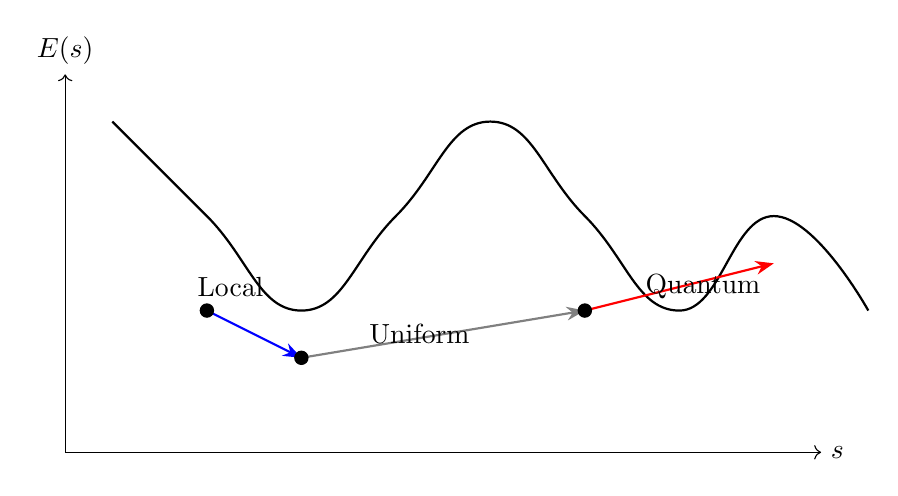
\begin{tikzpicture}[scale=1.2]
        % Draw the x-axis
        \draw[->] (0,0) -- (8,0) node[right] {$s$};
        % Draw the y-axis
        \draw[->] (0,0) -- (0,4) node[above] {$E(s)$};
        
        % Draw the energy function
        \draw[thick, smooth, tension=0.8] plot coordinates {
            (0.5, 3.5)
            (1.5, 2.5)
            (2.5, 1.5)
            (3.5, 2.5)
            (4.5, 3.5)
            (5.5, 2.5)
            (6.5, 1.5)
            (7.5, 2.5)
            (8.5, 1.5)
        };
        
        % Draw the local proposal arrow
        \draw[blue, thick, -Stealth] (1.5, 1.5) -- (2.5, 1);
        \node at (1.75, 1.75) {Local};
        
        % Draw the uniform proposal arrow
        \draw[gray, thick, -Stealth] (2.5, 1) -- (5.5, 1.5);
        \node at (3.75, 1.25) {Uniform};
        
        % Draw the quantum proposal arrow
        \draw[red, thick, -Stealth] (5.5, 1.5) -- (7.5, 2);
        \node at (6.75, 1.75) {Quantum};
        
        % Mark the starting point for the local proposal
        \filldraw[black] (1.5, 1.5) circle (2pt);
        
        % Mark the starting point for the uniform proposal
        \filldraw[black] (2.5, 1) circle (2pt);
        
        % Mark the starting point for the quantum proposal
        \filldraw[black] (5.5, 1.5) circle (2pt);
    \end{tikzpicture}
    \caption{Visualization of different candidate proposal techniques. The local one achieves relatively good acceptance rates while not exploring the state space. Uniform updating tries to explore the state space but struggles with acceptance since the proposed state has most likely high energy. However, the discussed quantum proposal routine samples states that are far away in the state space while having comparable energy, thus, also leading to high acceptance rates.}
    \label{fig:proposal_techniques}
\end{figure}

\end{document}